\documentclass[12pt]{article}

\usepackage[utf8]{inputenc}
\usepackage[T1]{fontenc}
\usepackage{datetime}
\usepackage[spanish]{babel}
\usepackage{graphicx}
\usepackage{listings}
\usepackage{caption}
\usepackage{subcaption}
\usepackage[right=2cm,left=2cm,top=2cm,bottom=2cm]{geometry}
\usepackage{hyperref}
\usepackage{fancyhdr}
\usepackage{color}
\usepackage[export]{adjustbox}
\usepackage{graphicx}
\usepackage{float}
\usepackage{changepage}
\usepackage{multicol}
\usepackage{imakeidx}
\usepackage{csquotes}
\usepackage{array}
\usepackage{tabularx}
\usepackage{xcolor}
\usepackage[backend=biber]{biblatex}
\addbibresource{webgrafia.bib}

\pagestyle{fancy}
\renewcommand{\footrulewidth}{0.4pt}
\setlength{\headheight}{15pt}


\fancyhead[L]{ CEIABD – SBD }
\fancyhead[R]{ Páez Anguita, Víctor }
\fancyfoot[L]{IES Gran Capitán}


\begin{document}

\begin{titlepage}
    \begin{center}
      \Large \bfseries{}
    \end{center}
    \vspace{0.1cm}
    \begin{center}
      \Large \bfseries{}
    \end{center}
    \vspace{0.1cm}
    \begin{center}
     \Large \bfseries{Análisis Comparativo de Herramientas de Procesamiento de Datos}
    \end{center}
    \vspace{0.0001cm}
    \begin{center}
        Departamento de informática \\ I.E.S. Gran Capitán - Córdoba
    \end{center}
        \vspace{2 cm}
\begin{figure}[h!]
    \centering
    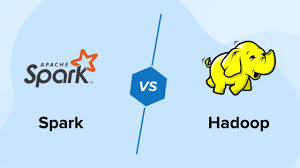
\includegraphics[width=.6\textwidth]{portada.png}
    \label{fig:my_label}
\end{figure}
    \vspace{0.2 cm}
    \begin{center}
        Inteligencia artificial y Big data \\ \currenttime 
    \end{center}
    \vspace{4 cm}
\null\hfill \textbf{Desarrollado por:}
\\
\\
\null\hfill Víctor Páez Anguita
\clearpage
\end{titlepage}

%%%%%%%%%%%%%%%%%%%%%%%%%%%Index%%%%%%%%%%%%%%%%%%%%%%%%%%%%%%%%
\tableofcontents
\clearpage
%%%%%%%%%%%%%%%%%%%%%%%%%%%Index%%%%%%%%%%%%%%%%%%%%%%%%%%%%%%%%

\section{Introducción}

El procesamiento de grandes volúmenes de datos ha impulsado el desarrollo de tecnologías como Apache Hadoop y Apache Spark. En los siguientes
puntos, se analizarán sus principales diferencias, casos de uso y ventajas comparativas.

\section{Hadoop}

Hadoop es un framework de código abierto que permite el procesamiento distribuido de grandes volúmenes de datos en clústeres de servidores. 
Fue creado por Doug Cutting y Mike Cafarella en 2005 y se basa en el modelo de programación MapReduce de Google. Hadoop es ampliamente utilizado en aplicaciones de Big Data y análisis de datos a gran escala.

\subsection{Arquitectura}
Hadoop se compone de cuatro módulos principales:
\begin{itemize}
    \item \textbf{Hadoop Distributed File System (HDFS):} Un sistema de archivos distribuido que permite el almacenamiento de grandes volúmenes de datos dividiéndolos en bloques distribuidos en varios nodos.
    \item \textbf{Yet Another Resource Negotiator (YARN):} Administra los recursos del clúster y la ejecución de tareas de procesamiento.
    \item \textbf{MapReduce:} Un modelo de programación para el procesamiento paralelo de grandes conjuntos de datos.
    \item \textbf{Hadoop Common:} Contiene las bibliotecas y utilidades necesarias para que los otros módulos funcionen correctamente.
\end{itemize}

\begin{figure}[h!]
    \centering
    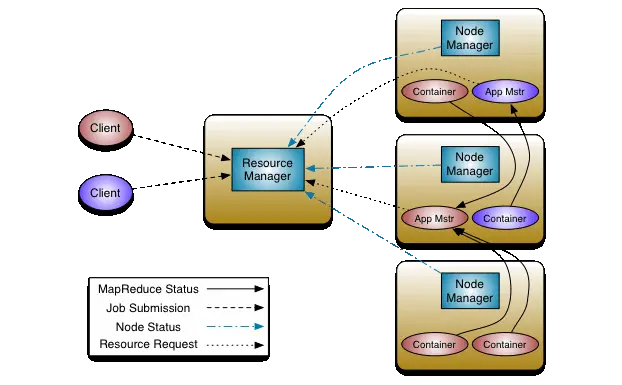
\includegraphics[width=.7\textwidth]{esquema-hadoop.png}
    \label{fig:my_label}
\end{figure}

\subsection{Ventajas}
\begin{itemize}
    \item Escalabilidad horizontal mediante la adición de nuevos nodos al clúster.
    \item Alta tolerancia a fallos gracias a la replicación de datos en múltiples nodos.
    \item Flexibilidad para manejar datos estructurados y no estructurados.
    \item Costo reducido al utilizar hardware convencional.
\end{itemize}

\subsection{Desventajas}
\begin{itemize}
    \item Latencia en el procesamiento debido al modelo de ejecución batch de MapReduce.
    \item Complejidad en la configuración y administración del clúster.
    \item Requiere conocimientos avanzados en programación para su implementación óptima.
\end{itemize}

\subsection{Aplicaciones}
Hadoop es ampliamente utilizado en diversos sectores:
\begin{itemize}
    \item \textbf{Empresas de tecnología:} Facebook y Yahoo lo usan para el procesamiento y análisis de grandes volúmenes de datos de usuarios.
    \item \textbf{Sector financiero:} Bancos y aseguradoras lo emplean para la detección de fraudes y análisis de riesgos.
    \item \textbf{Salud:} Hospitales y laboratorios lo aplican en el análisis de datos genómicos y epidemiológicos.
\end{itemize}

\subsection{Procesamiento de datos en Hadoop}

\subsubsection{Batch}
Hadoop implementa el procesamiento batch a través de MapReduce, donde los datos se leen en grandes volúmenes, se procesan en múltiples etapas y se almacenan nuevamente en HDFS. Este enfoque es ideal para tareas como agregaciones masivas y análisis históricos.

\subsubsection{Streaming}
Hadoop permite el procesamiento de datos en streaming mediante herramientas como Apache Flume y Apache Kafka, que recopilan y envían datos en tiempo real para ser procesados mediante frameworks como Apache Storm o Spark Streaming.

\subsubsection{En tiempo real}
Si bien Hadoop no está diseñado para procesamiento en tiempo real, su integración con Apache Spark permite realizar análisis en memoria con latencias mucho más bajas en comparación con MapReduce. Esto es útil en aplicaciones como detección de fraudes y análisis de redes sociales en tiempo real.



\section{Spark}

Spark es un framework de procesamiento de datos en memoria que permite el análisis de grandes volúmenes de datos de forma rápida y eficiente. 
Fue desarrollado por el AMPLab de la Universidad de California, Berkeley, y se basa en el modelo de programación MapReduce de Hadoop. Spark es ampliamente utilizado en aplicaciones de Big Data y machine learning.

\subsection{Arquitectura}
Spark se compone de los siguientes módulos:
\begin{itemize}
    \item \textbf{Spark Core:} Motor principal de ejecución y gestión de tareas.
    \item \textbf{Spark SQL:} Soporte para consultas SQL sobre grandes volúmenes de datos.
    \item \textbf{Spark Streaming:} Procesamiento en tiempo real de flujos de datos.
    \item \textbf{MLlib:} Biblioteca de aprendizaje automático.
    \item \textbf{GraphX:} Procesamiento de datos en forma de grafos.
\end{itemize}

\begin{figure}[h!]
    \centering
    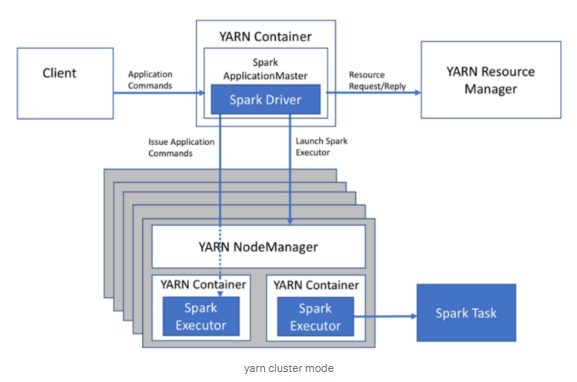
\includegraphics[width=.7\textwidth]{esquema-spark.png}
    \label{fig:my_label}
\end{figure}

\subsection{Ventajas}
\begin{itemize}
    \item Procesamiento en memoria para mayor velocidad.
    \item Soporte para múltiples lenguajes de programación.
    \item Integración con diversas herramientas de Big Data.
    \item Facilidad de uso con APIs amigables.
\end{itemize}

\subsection{Desventajas}
\begin{itemize}
    \item Mayor consumo de memoria en comparación con Hadoop.
    \item No es óptimo para almacenamiento de datos.
    \item Dependencia en sistemas de almacenamiento externos como HDFS.
\end{itemize}

\subsection{Aplicaciones}
\begin{itemize}
    \item \textbf{Netflix:} Optimización de recomendaciones en tiempo real.
    \item \textbf{Uber:} Análisis y optimización de rutas en tiempo real.
    \item \textbf{Banca:} Detección de fraudes con análisis en streaming.
\end{itemize}

\subsection{Procesamiento de datos en Spark}

\subsubsection{Batch}
Spark permite el procesamiento batch mediante Spark Core y Spark SQL, facilitando el análisis de grandes volúmenes de datos almacenados en HDFS, Amazon S3 o bases de datos distribuidas.

\subsubsection{Streaming}
Spark Streaming permite el procesamiento en tiempo real de datos provenientes de fuentes como Apache Kafka, Flume o sockets de red, utilizando micro-batching para mejorar la eficiencia.

\subsubsection{En tiempo real}
Con la introducción de Structured Streaming, Spark proporciona procesamiento en tiempo real con una latencia mínima, ideal para aplicaciones como monitoreo de redes, detección de fraudes y análisis de comportamiento de usuarios.


\section{Comparativa}

\begin{itemize}
    \item \textbf{Velocidad:} Spark es hasta 100 veces más rápido que Hadoop en ciertos procesos debido a su capacidad de procesamiento en memoria, mientras que Hadoop se basa en discos, lo que lo hace más lento.
    \item \textbf{Facilidad de uso:} Spark proporciona APIs en varios lenguajes de programación como Scala, Python y Java, lo que facilita su adopción, mientras que Hadoop requiere programación más detallada con MapReduce.
    \item \textbf{Gestión de datos:} Hadoop es más adecuado para el almacenamiento y procesamiento batch de grandes volúmenes de datos, mientras que Spark está diseñado para cálculos en memoria y procesamiento rápido.
    \item \textbf{Costo y hardware:} Hadoop puede ejecutarse en hardware convencional, lo que reduce costos, mientras que Spark requiere máquinas con alta capacidad de memoria RAM para un rendimiento óptimo.
    \item \textbf{Casos de uso:} Hadoop es ideal para almacenamiento masivo y análisis de datos históricos, mientras que Spark se adapta mejor a aplicaciones que requieren procesamiento en tiempo real, como análisis de redes sociales y detección de fraudes.
    \item \textbf{Integración:} Ambas tecnologías pueden utilizarse en conjunto; Spark puede usarse para procesamiento rápido sobre datos almacenados en HDFS de Hadoop.
\end{itemize}

\begin{figure}[h!]
    \centering
    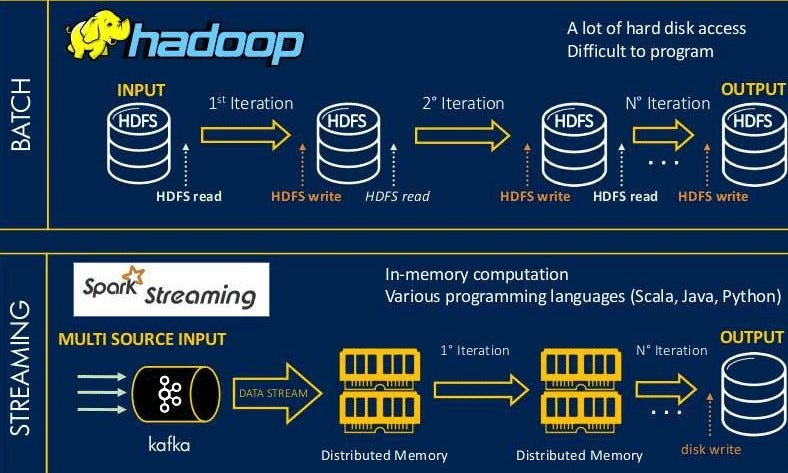
\includegraphics[width=.7\textwidth]{comparativa.jpg}
    \label{fig:my_label}
\end{figure}

\clearpage

\section{Conclusión}

Ambas tecnologías tienen aplicaciones distintas y su elección depende de los requisitos específicos del proyecto. 
Mientras Hadoop es ideal para almacenamiento y procesamiento batch, Spark es preferido para análisis rápidos y procesamiento en memoria.

\clearpage

\section{Webgrafia}


Hadoop
\\
Arquitectura
\\
\cite{aprenderbigdata-hadoop}
\cite{ionos-hadoop}
\\
Ventajas y desventajas
\\
\cite{hostzealot-hadoop}
\cite{jacagudelo-hadoop}
\\
Aplicaciones comúnes
\\
\cite{powerdata-hadoop}
\\
Procesamiento de datos en hadoop
\\
\cite{deusto-hadoop}
\\
\\
Spark
\\
Arquitectura
\\
\cite{keepcoding-spark}
\cite{medium-spark}
\\
Ventajas y desventajas
\\
\cite{bbvaapimarket-spark}
\cite{ionos-spark}
\\
Aplicaciones comúnes en Spark
\\
\cite{googleCloud-spark}
\\
Procesamiento de datos en Spark
\\
\cite{diegocalvo-spark}
\\

Comparativa de Hadoop y Spark
\\
\cite{aws-hadoop-spark}
\cite{esic-hadoop-spark}
\cite{inesdi-hadoop-spark}
\cite{hadoop-spark}

\printbibliography

\end{document}
